% 11 --------------------------------------------------------------------------
\begin{frame}{What Does a Lloyd Fixed Point Guarantee?}
  \footnotesize
  \begin{columns}[T,onlytextwidth]
    \column{.46\textwidth}
      \textbf{For arbitrary initialization}
      \begin{itemize}\setlength{\itemsep}{.06cm}
        \item With deterministic tie-breaking, SSE is non-increasing and the finite assignment set leads to a fixed point.
        \item A fixed point is stationary under the two Lloyd updates, not globally optimal.
        \item Arbitrary Lloyd starts have \textcolor{red}{no} finite worst-case approximation ratio.
      \end{itemize}
    \column{.46\textwidth}
      \textbf{What initialization can add}
      \begin{itemize}\setlength{\itemsep}{.06cm}
        \item k-means++ [AV2007] gives
        \[
          \E[J_{\mathrm{init}}]\le 8(\ln K+2)\,J^*.
        \]
        \item Lloyd iterations only decrease $\phi$, so the same expected upper bound holds for the final run.
        \item Computing $J^*$ is l NP-hard in the general case.
      \end{itemize}
  \end{columns}
  \vspace{0.5cm}
  \scriptsize [AV2007]  k-means++: The Advantages of Careful Seeding. David Arthur and Sergei Vassilvitskii, SODA 2007, pp. 1027–1035.
\end{frame}

% 12 ------------------------------------------------------------------

% 13 --------------------------------------------------------------------------
\begin{frame}{Initialization Is Part of the Algorithm}
  \begin{columns}[T,onlytextwidth]
    \column{.47\textwidth}
      \textbf{Random starts}
      \begin{itemize}\spaceditems
        \item Simple, but centers may start together.
        \item A single seed can be misleading.
      \end{itemize}
    \column{.47\textwidth}
      \textbf{k-means++}
      \begin{itemize}\spaceditems
        \item Choose the first center at random.
        \item Sample later centers with probability proportional to squared distance from the current set.
      \end{itemize}
  \end{columns}
  \pause
  \vspace{.5cm}
  \begin{tikzpicture}
    \node[greenbox,text width=10.3cm] {In practice: use k-means++, several restarts, a fixed seed for reproducibility, and report the spread of final objectives.};
  \end{tikzpicture}
\end{frame}

% 12 --------------------------------------------------------------------------
\begin{frame}{Implementation Details Change the Result}

      \begin{itemize}\spaceditems
        \item Standardize or transform features before measuring distances.
        \item Decide how to handle missing values and empty clusters.
        \item Remove or robustly treat influential outliers.
           \item Use MiniBatchKMeans when one full pass is too expensive.
      \end{itemize}

\end{frame}

% 13 ------------------------------------------------------------------
% 14 --------------------------------------------------------------------------
\begin{frame}{How Should We Choose $K$?}
  \begin{columns}[T,onlytextwidth]
    \column{.46\textwidth}
      \textbf{Inertia}
      \[
        \operatorname{inertia}(K)=\min_{z,\mu}J(z,\mu).
      \]
      It never increases as $K$ grows.
    \column{.46\textwidth}
      \textbf{Silhouette}
      \[
        s_i=\frac{b_i-a_i}{\max(a_i,b_i)}.
      \]
      Compare within-cluster and nearest-other-cluster distances.
  \end{columns}
  \vspace{.5cm}
  \small
  \begin{itemize}
  	\item $a_i$:  the average distance to the datapoints within the same clique  $\frac{1}{ |C_i|-1} \sum_{j\in C_i, j\neq i} \|x_i - x_i\|$
  	\item $b_i$:  the minimal average distance to a neighbor clique $\min_{C\neq C_i} \frac{1}{|C|} \sum_{j\in C} \| x_i- x_j\|$.
  \end{itemize}
\end{frame}

% 15 --------------------------------------------------------------------------
\begin{frame}{A Low Inertia Is Not Always Good}
  \begin{columns}[c,onlytextwidth]
    \column{.48\textwidth}
      \begin{tikzpicture}[x=.46cm,y=.42cm]
        \draw[->] (0,0)--(8.8,0) node[right]{$K$};
        \draw[->] (0,0)--(0,6.1) node[above]{inertia};
        \draw[thick,forestgreen] plot[smooth] coordinates {(1,5.5)(2,3.2)(3,2.2)(4,1.8)(5,1.6)(6,1.48)(7,1.4)(8,1.34)};
      \end{tikzpicture}
    \column{.46\textwidth}
      \begin{itemize}\spaceditems
        \item Increasing $K$ always improves the training objective.
        \item A stable cluster across seeds or resamples is more credible.
        \item A useful cluster must have an interpretable consequence.
      \end{itemize}
  \end{columns}
\end{frame}

% 16 --------------------------------------------------------------------------
\begin{frame}{Failure Gallery: The Geometry Is the Model}
  \begin{columns}[T,onlytextwidth]
    \column{.31\textwidth}
      \centering
      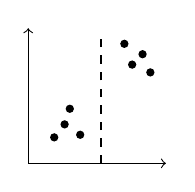
\begin{tikzpicture}[x=.33cm,y=.33cm]
        \draw[->] (0,0)--(5.3,0);\draw[->] (0,0)--(0,5.2);
        \foreach \x/\y in {1/1,1.4/1.5,2/1.1,1.6/2.1,4/3.8,4.4/4.2,3.7/4.6,4.7/3.5}{\fill[black] (\x,\y) circle (1.5pt);}
        \draw[dashed] (2.8,0)--(2.8,5);
      \end{tikzpicture}
      \par\small Well-separated blobs
    \column{.31\textwidth}
      \centering
      \begin{tikzpicture}[x=.33cm,y=.33cm]
        \draw[->] (0,0)--(5.3,0);\draw[->] (0,0)--(0,5.2);
        \draw[thick,forestgreen] (0.8,1.3) .. controls (1.6,2.8) and (3.6,2.8) .. (4.5,1.3);
        \draw[thick,slideorange] (0.8,3.9) .. controls (1.6,2.4) and (3.6,2.4) .. (4.5,3.9);
      \end{tikzpicture}
      \par\small Non-convex structure
    \column{.31\textwidth}
      \centering
      \begin{tikzpicture}[x=.33cm,y=.33cm]
        \draw[->] (0,0)--(5.3,0);\draw[->] (0,0)--(0,5.2);
        \foreach \x/\y in {1/1,1.5/1.2,1.3/1.8,4/2.6,4.3/2.9,4.5/3.3,2.1/4.4}{\fill[black] (\x,\y) circle (1.5pt);}
        \fill[warningred] (2.1,4.4) circle (2.6pt);
      \end{tikzpicture}
      \par\small Unequal density and outliers
  \end{columns}
  \vspace{.45cm}
  \centering
  When K-means fails, ask whether the distance, scale, $K$, or cluster shape is mismatched to the data.
\end{frame}

% 17 --------------------------------------------------------------------------
\begin{frame}{Complexity and Scaling to Larger Data}
  Total computational cost $O(nKdt)$.
  \begin{itemize}
  	\item $n$: the size of dataset;
  	\item $K$: the number of clusters;
  	\item $d$: feature dimension;
  	\item $t$:  number of iteration steps.
  \end{itemize}
  \vspace{0.3cm}
  \pause
  Approaches for scaling up
      \begin{itemize}\spaceditems
        \item Mini-batches reduce the cost of each update.
        \item Sparse or approximate distance routines reduce memory pressure.
      \end{itemize}
\end{frame}
